\begin{frame}
  \frametitle{L�gicas modales}
  \begin{center} $ p \equiv "$Hoy hace fr�o$"$ \end{center}
  \visible<2->{
    \begin{itemize}
    \item �Hace realmente fr�o?
    \item �Es sabido que hoy hace fr�o?
    \item �Hace fr�o ahora, o dentro de un rato?
    \item Si vuelo a Dubl�n, �seguir� haciendo fr�o?
    \end{itemize}
  }
\end{frame}

%===================================
\sectionDark{L�gica epist�mica} %===
% ===================================
\begin{frame}
  \frametitle{L�gica epist�mica (1 agente)}
  \vspace{0.8cm}
  \begin{columns}
    \begin{column}{0.5\textwidth}
      L�gica proposicional:
      \begin{itemize}
      \item $p, q, \cdots \in \mathcal{P}$
      \item $\varphi,\quad \neg\varphi,\quad \varphi\mor\psi,\quad \varphi\mand\psi$
      \item $\varphi \rightarrow \psi $ ( $\myeq \neg\varphi \mor \psi$ )
      \end{itemize}
    \end{column}
    \begin{column}{0.5\textwidth}
      \visible<2->{
        L�gica epist�mica:
        \begin{itemize}
        \item $\K\,\varphi$\hspace{2.5cm}
        \item $\M\,\varphi \myeq \neg\K\neg\varphi$\hspace{0.9cm}
        \end{itemize}
      }
    \end{column}
  \end{columns}
  \vspace{1cm}
  \visible<3->{
    \begin{align*}
      \K(\varphi \rightarrow \psi): & \hspace{0.3cm} \text{``Se sabe que }
                                      \varphi \text{ implica } \psi\text{'' }\\
      \K \varphi \mor \K \neg \varphi: & \hspace{0.3cm} \text{``Se sabe que }
                                         \varphi \text{ o }
                                         \neg\varphi\text{'' } \\
      \K \varphi \mor \neg \K \varphi:  &\hspace{0.3cm} \text{``Puede que se sepa
                                          o no que }\varphi \text{'' } \\
    \end{align*}
  }
\end{frame}


\begin{frame}
  \frametitle{Modelo de mundos posibles}
  \begin{center}{ $ \MM =\,< W, R, V >$}\end{center}

     $W = \{w_1, w_2, w_3, \ldots \}$ : Conjunto de mundos (o estados)
     posibles. \\
     $R =  \prescript{}{i}{R}_j$ : Operador de relaci�n entre mundos (o estados). \\


  \begin{block}{Ejemplo:}
    \begin{minipage}{.4\linewidth}%
      $p = $ ``Hoy es viernes''\\
      $q = $ ``Hoy es s�bado''\\
    \end{minipage}%
    \begin{minipage}{.6\linewidth}%
    \end{minipage}%
  \end{block}
\end{frame}

\sectionDarkSpecial{Ejemplo}
\begin{frame}
  \frametitle{Ejemplo}
  
  \begin{columns}
    \begin{column}{0.55\textwidth}
      Suponemos que existen \alert{tres cartas} (1, 2 y 3):\\
      -- Alicia tiene una carta en la mano.\\
      -- Otra bocabajo en la mesa.\\
      -- La �ltima se devuelve al mont�n.\\
      
      \vspace{0.5cm}
      \only<1,2>{\textbf{�Cu�les son los estados relevantes?}}
      \only<3,4,5>{\textbf{�Qu� informaci�n tiene Alicia?}}
      \only<6->{
        $H_i \myeq $ ``Alicia tiene la carta $i$''\\
        $T_i \myeq $ ``La carta $i$ est� en la mesa''\\
      }
    \end{column}
    \begin{column}{0.55\textwidth}
      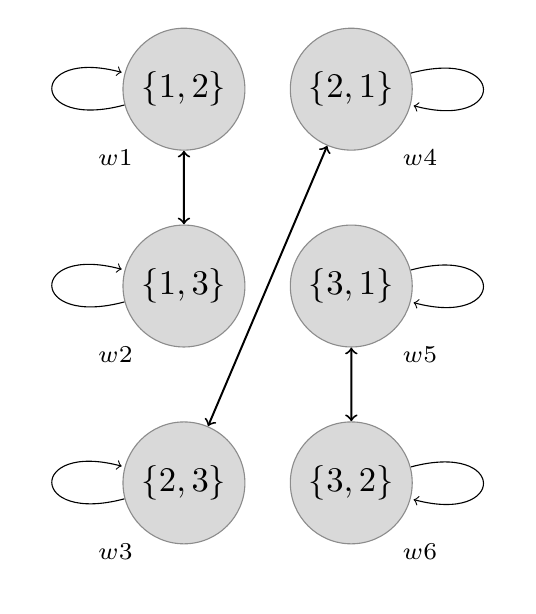
\begin{tikzpicture}[scale=1.25, transform shape]
        \visible<2->{
          \tikzstyle{every node} = [circle, fill=gray!30, draw=gray!90] 
          \node [label=below left:\scriptsize$w1$] (w1) at (0.0, 4.0) {$\{1,2\}$};
          \node [label=below right:\scriptsize$w4$] (w4) at (1.7, 4.0) {$\{2,1\}$};
          \node [label=below left:\scriptsize$w2$] (w2) at (0.0, 2.0) {$\{1,3\}$};
          \node [label=below right:\scriptsize$w5$] (w5) at (1.7, 2.0) {$\{3,1\}$};
          \node [label=below left:\scriptsize$w3$] (w3) at (0.0, 0.0) {$\{2,3\}$};
          \node [label=below right:\scriptsize$w6$] (w6) at (1.7, 0.0) {$\{3,2\}$};
          \visible<4->{
            \draw [line width = 0.25mm, <->] (w1) -- (w2);
            \draw [line width = 0.25mm, <->] (w3) -- (w4);
            \draw [line width = 0.25mm, <->] (w5) -- (w6);
          }
          \visible<5->{
            \path [->] (w1) edge[loop left] ();
            \path [->] (w2) edge[loop left] ();
            \path [->] (w3) edge[loop left] ();
            \path [->] (w4) edge[loop right] ();
            \path [->] (w5) edge[loop right] ();
            \path [->] (w6) edge[loop right] ();
          }
        }
      \end{tikzpicture}
    \end{column}
  \end{columns}
\end{frame}




%
%
%%%
%%% Local Variables:
%%% mode: latex
%%% TeX-master: "./carcasa.tex"
%%% End:
